\documentclass[letterpaper, 10pt]{article}

\usepackage{fancyhdr}
\usepackage[left=2.35cm,top=2.45cm,bottom=2.45cm,right=2.35cm,letterpaper]{geometry}
\usepackage{amsmath}
\usepackage{graphicx}

\pagestyle{fancy}
\fancyhf{}
\fancyfoot[C,CO]{\thepage}
\fancyhead[L,LO]{\bfseries EECS 233} %Class Title
\fancyhead[C,CO]{\bfseries Homework \#1} %Assignment Title
\fancyhead[R,RO]{\bfseries Fall 2016} %Semester 

\newenvironment{questions}{ \noindent \textbf{Questions}} %BoldFaced Subsection

\newenvironment{q1}{\noindent Question 1:} %Question Number

\newenvironment{a1}{\noindent } %Answer

\newenvironment{q2}{\noindent Question 2:}

\newenvironment{a2}{\noindent } %Answer

\newenvironment{q3}{\noindent Question 3:}

\newenvironment{a3}{\noindent } %Answer

\newenvironment{q4}{\noindent Question 4:}

\newenvironment{a4}{\noindent } %Answer

\newenvironment{Example1}{\noident Example1:}

\newenvironment{Example2}{\noident Example2:}

\newenvironment{Example3}{\noident Example3:}

\newenvironment{Example4}{\noident Example4:}

\begin{document}
	
	\noindent
	Andrew Covarrubias (axc554) %Name
	\bigskip
	\bigskip
	
	\begin{questions} %Start Questions
		
		\bigskip
		
		\begin{q1} %Question
			\\
			\textbf{
				What are the results for each of the programs? In your report, include the program name, and copy/paste the output.}
			
		\end{q1}
		
		\bigskip
		
		\begin{a1} %Answer
			
			\begin{Example1}
				\\
				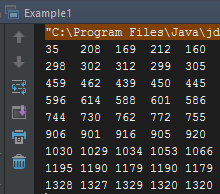
\includegraphics{Example1}
				
			\end{Example1}
			
			\begin{Example2}
				\\
				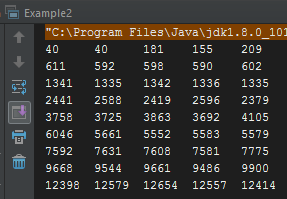
\includegraphics{Example2}
			\end{Example2}
			
			\begin{Example3}
				\\
				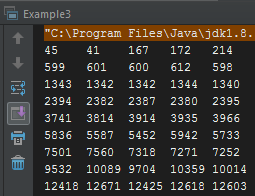
\includegraphics{Example3}
			\end{Example3}
			
			\newpage
			
			\begin{Example4}
				\\
				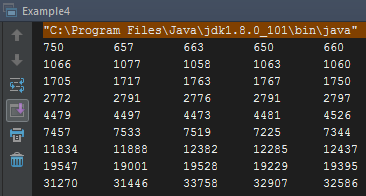
\includegraphics{Example4}
			\end{Example4}
			
		\end{a1}
		
		\bigskip
		
		\begin{q2} %Question
			\\
			\textbf{
				Explain (in complete sentences) how each algorithm compares quantitatively. How much faster does the time grow for each algorithm as compared to the others?}
			
		\end{q2}
		
		\bigskip
		
		\begin{a2} %Answer
			The four different examples each use different algorithms which all vary in speed.\\
			\\
			In order of speed Example1 is the fastest and Example4 is the slowest, the order being Example1, Example2, Example3, Example4 and the time growth is the reverse Example4 grows the quickest and Example1 grows the slowest.\\
			\\
			Example1 has a linear run time of n, where each value is run through one time due to the single loop\\
			\\
			Example2 has a squared run time of $n^2$, where each value is run through two times because of the nested for loops. Example2 will grow at a rate of Example1 squared\\
			\\
			Example3 has a cubed run time of $n^3$. This is due to it being a combination of Example1 and Example2. It has both a single for loop which runs through all the values and a nested for loop which runs through each value twice. As a result the run time can be shown by the following equation $n^3 = n^2 * n$. Example3 will grow at a rate of Example3 cubed.\\
			\\
			Example4 has an exponential run time of $2^n$ meaning it will undoubtedly take the longest. It's run time comes from the recursive method it calls itself. Meaning for a given n value the previous two n values are required and the process repeats itself for however large the n value is. 
		\end{a2}
		\bigskip
		
		\begin{q3} %Question
			\\
			\textbf{
				What do you notice about the results that might be unexpected?}
			
		\end{q3}
		
		\bigskip
		
		\begin{a3} %Answer
			For the Example1 and Example2 it seemed to be that the first few values were always lower than the rest of the values. It seemed to repeat, where the first few trials of the initial n values would be lower than the later trials. For instance Example1 starts with 35 and the rest of the values are above 150. 
		\end{a3}
		\bigskip
		
		\begin{q4} %Question
			\\
			\textbf{Offer a possible explanation for the unexpected results in Question (3) above.}
			
		\end{q4}
		
		\bigskip
		
		\begin{a4} %Answer
			After thinking about it for a while I could not really think of a reasonable explanation for the unexpected results. The only thing that might have gone wrong was the way I used for loops to print all the trials with different n values. I tried playing around with the placement of the loops and time counting, but nothing seemed to work. 
		\end{a4}
		
		
	\end{questions}
\end{document}
